In this section we describe the experimental results we have obtained using Cerebro and the associated tools. We conduct
tests using five sample applications. 

\begin{description}
\item[StudentInfo] A JAXRS application for managing students of a class. Provides APIs for
adding/removing students, and listing the student information.
\item[ServerHealth] An application that monitors a given web URL for server uptime. Provides an
API for obtaining the uptime statistics computed by the application.
\item[SocialMapper] A simple social networking application. Provides APIs for adding users,
comments and other resources.
\item[StockTrader] A stock trading application. Provides APIs for adding users, registering
companies, buying and selling stocks among users.
\item[Rooms] A hotel booking application. Provides APIs for registering hotels and looking up
available rooms.
\end{description}

The above applications extensively use the datastore cloud SDK operations of Google App Engine. The Rooms application
additionally uses the memcache cloud SDK operations.

We instrument each of the five sample applications to measure the time taken by their web APIs to execute the
enclosed code. This is done by adding some extra Java code to each of the web APIs exposed by the sample applications.
We ensure that the instrumentation does not alter the original web API code in anyway (i.e. the original algorithms, control flow
and data flow are not impacted by the instrumentation). Then for each application we also
implement a mechanism to output the measured execution times, so an external client can query and collect the execution
times of the web APIs.

We carry out each of our tests in two separate environments -- Google App Engine public cloud, and
the AppScale private cloud. The AppScale private cloud used for testing was powered by four m3.2xlarge virtual machines 
running on a private Eucalyptus cluster.

In the first set of experiments, we benchmark each application for a period of 15 to 20 hours.
During this time, we run an HTTP client on a separate machine that invokes the instrumented web APIs once every minute, 
and collects the server-side execution times (as measured by the instrumentation code).
At the same time, we also run Watchtower in the same target cloud environment as the sample application being tested to
benchmark the individual cloud SDK operations. Recall that our sample applications use datastore and memcache
cloud SDK operations. Hence
we configure Watchtower to periodically benchmark the cloud SDK operations related to datastore and memcache. 
At the end of a benchmarking run, we have two sets of data at hand:

\begin{itemize}
\item Web API execution times collected by the benchmarking HTTP client
\item Cloud SDK benchmarking data gathered by Watchtower
\end{itemize}

We now run Cerebro to make predictions regarding the web API execution time using the cloud SDK benchmarking data
collected by Watchtower. We configure Cerebro to predict an upper bound for the 95th percentile of the web API
execution time, with an upper confidence of 0.01. Cerebro generates a sequence of execution time predictions -- one 
per minute. Then we compare these predictions against the actual web API execution times collected during the same
time period. More specifically, we approximately align the sequence of predictions with the time series of actual execution
times, and check whether each prediction is correct (i.e. prediction is equal to or higher than the
corresponding actual value). We then use the results to compute a running tally of the percentage accuracy of Cerebro
predictions over time.

\begin{figure}
\centering
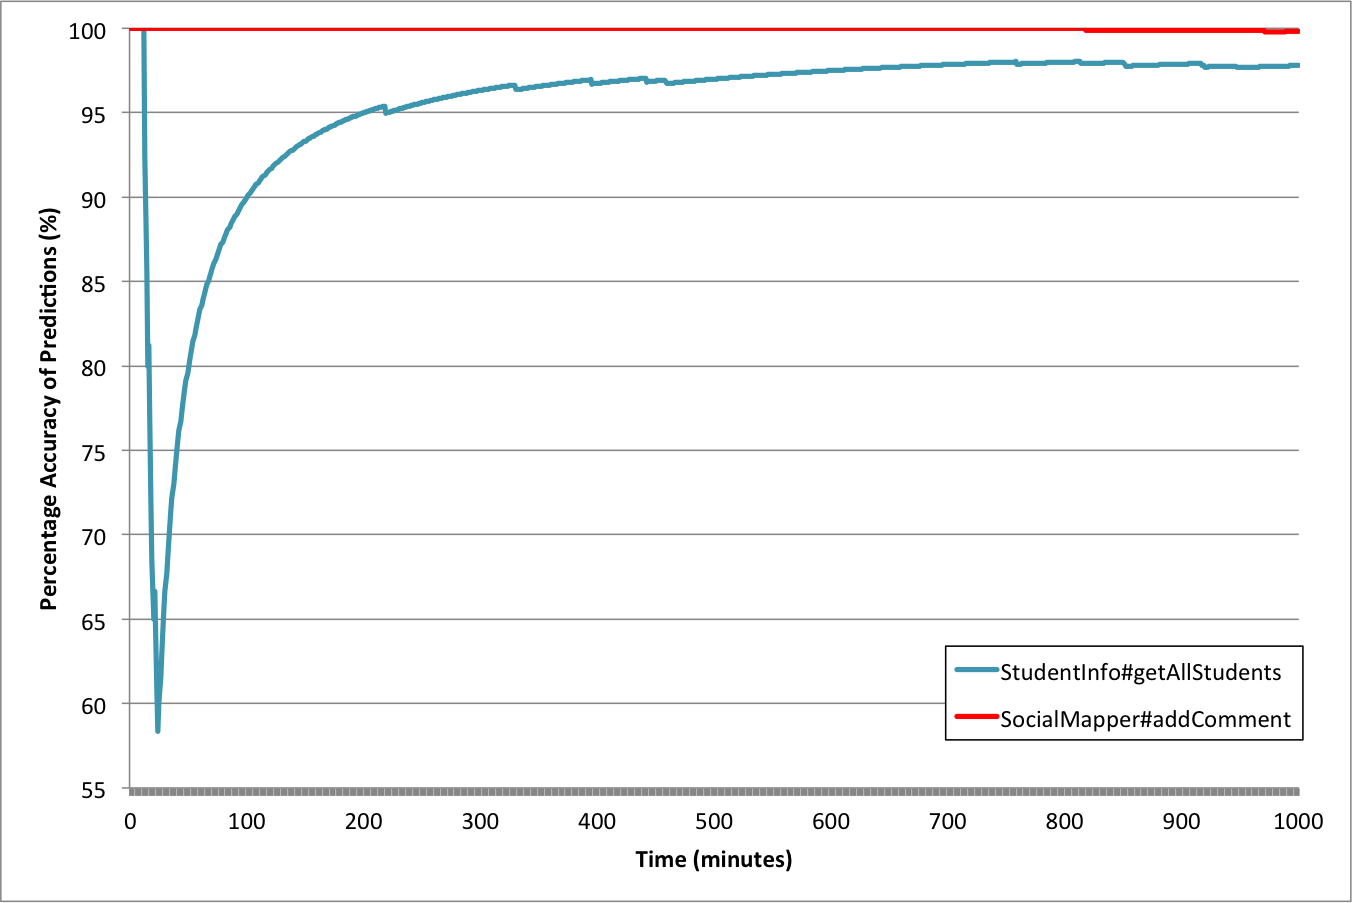
\includegraphics[scale=0.35]{gae_accuracy}
\caption{Percentage accuracy of predictions made on Google App Engine.}
\label{fig:gae_accuracy}
\end{figure}

\begin{figure}
\centering
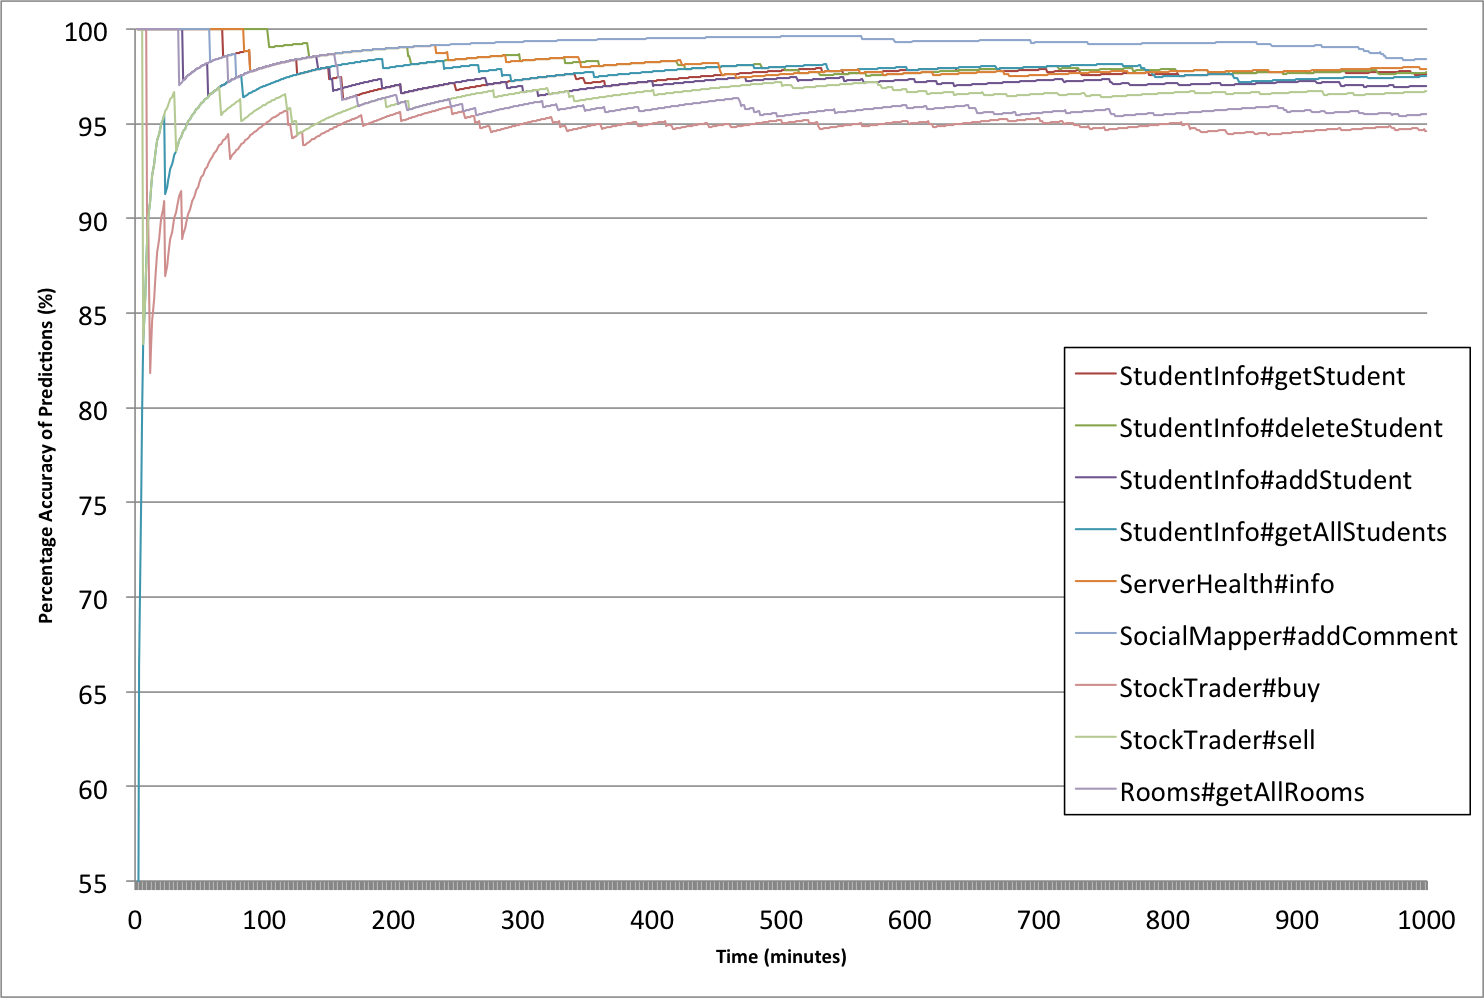
\includegraphics[scale=0.35]{as_accuracy}
\caption{Percentage accuracy of predictions made on AppScale.}
\label{fig:as_accuracy}
\end{figure}

Figure~\ref{fig:gae_accuracy} shows the percentage accuracy of the Cerebro predictions made in the Google App Engine 
public cloud environment. Each of the curves correspond to a single web API operation in one of the sample applications. 
The curves are labeled in the form of \textit{ApplicationName\#OperationName}. To maintain clarity in the figures we do not 
illustrate the results for all web API operations in the sample applications. Instead we present the results for a selected set of 
web API operations covering all five sample applications. We note that other web API operations we tested also produce
very similar results.

As expected QBETS takes some time to learn
from the time series data captured by Watchtower. This is when we see large fluctuations in the percentage accuracy. But
once QBETS has converged it consistently produces highly accurate predictions regarding the 95th percentile of the web API
response time. In the worst case QBETS takes up to 200 minutes to converge. This is the case with the
StudentInfo\#getAllStudents operation. After 275 minutes, we see highly accurate predictions being made on all web API
operations considered in the tests. After this point, we consistently see percentage accuracy values higher than 96\%. Note that
we had configured Cerebro to predict the 95th percentile of the web API executions time. Therefore as long as Cerebro produces
results with a percentage accuracy close to or higher than 95\%, we can consider the predictions to be correct and reliable.

The web API operations illustrated in figure~\ref{fig:gae_accuracy} cover a wide spectrum of scenarios that may be encountered
when statically analyzing web application code. StudentInfo\#getStudent and StudentInfo\#addStudent are by far the simplest
operations in the mix. They invoke a single cloud SDK operation each, and represent a simple database read scenario and a simple
database write scenario respectively. As per our survey on the cloud applications, these alone cover a significant portion of the 
web APIs developed for the Google App Engine and AppScale cloud platforms (1 path through the code, and 1 cloud SDK call). 
The StudentInfo\#deleteStudent operation makes two cloud SDK operations in sequence, whereas
StudentInfo\#getAllStudents performs a batch read from the datastore followed by a data dependent loop to iterate through the results.
In our experiment involving the StudentInfo\#getAllStudents operation, we had the datastore preloaded with 1000 student records, 
and Cerebro was configured to use a maximum entity count of 1000 when making predictions.

ServerHealth\#info invokes the same cloud SDK operation three times in sequence. Both StockTrader\#buy and StockTrader\#sell have
multiple paths through the code (due to branching), thus causing Cerebro to make multiple sequences of predictions -- one sequence
per path. The results shown in figure~\ref{fig:gae_accuracy} are for the longest paths which consist of seven cloud SDK invocations each. According to
our survey, 99.8\% of the execution paths found in Google App Engine applications have seven or less cloud SDK calls in them. Therefore we believe
that the web API operations in StockTrader application represent an important upper bound case. Rooms\#getRoomByName
invokes two different cloud SDK interfaces, namely datastore and memcache. Rooms\#getAllRooms is another operation that consists of
a loop. It is encouraging to see how Cerebro manages to produce highly accurate predictions for such a wide range of web API implementations.

Figure 2 shows the same results calculated by running the sample applications and the Watchtower in the AppScale private cloud
environment. [More content to Follow -- some experiments still in progress]

\subsection{Tightness of Predictions}
In this section we discuss the tightness of the predictions generated by Cerebro. Tightness is a measure of how closely the predictions
reflect the actual response times of web APIs. This parameter is just as important as the percentage accuracy of the predictions (which 
was discussed in the previous section). Note that Cerebro can achieve a very high percentage accuracy level by simply generating a 
sequence of absurdly large predictions. But such results will obviously be of very little use to the cloud administrators and API
developers. For the predictions to be useful and even meaningful, they should be very close to the actual response times of the web APIs.

\begin{figure}
\centering
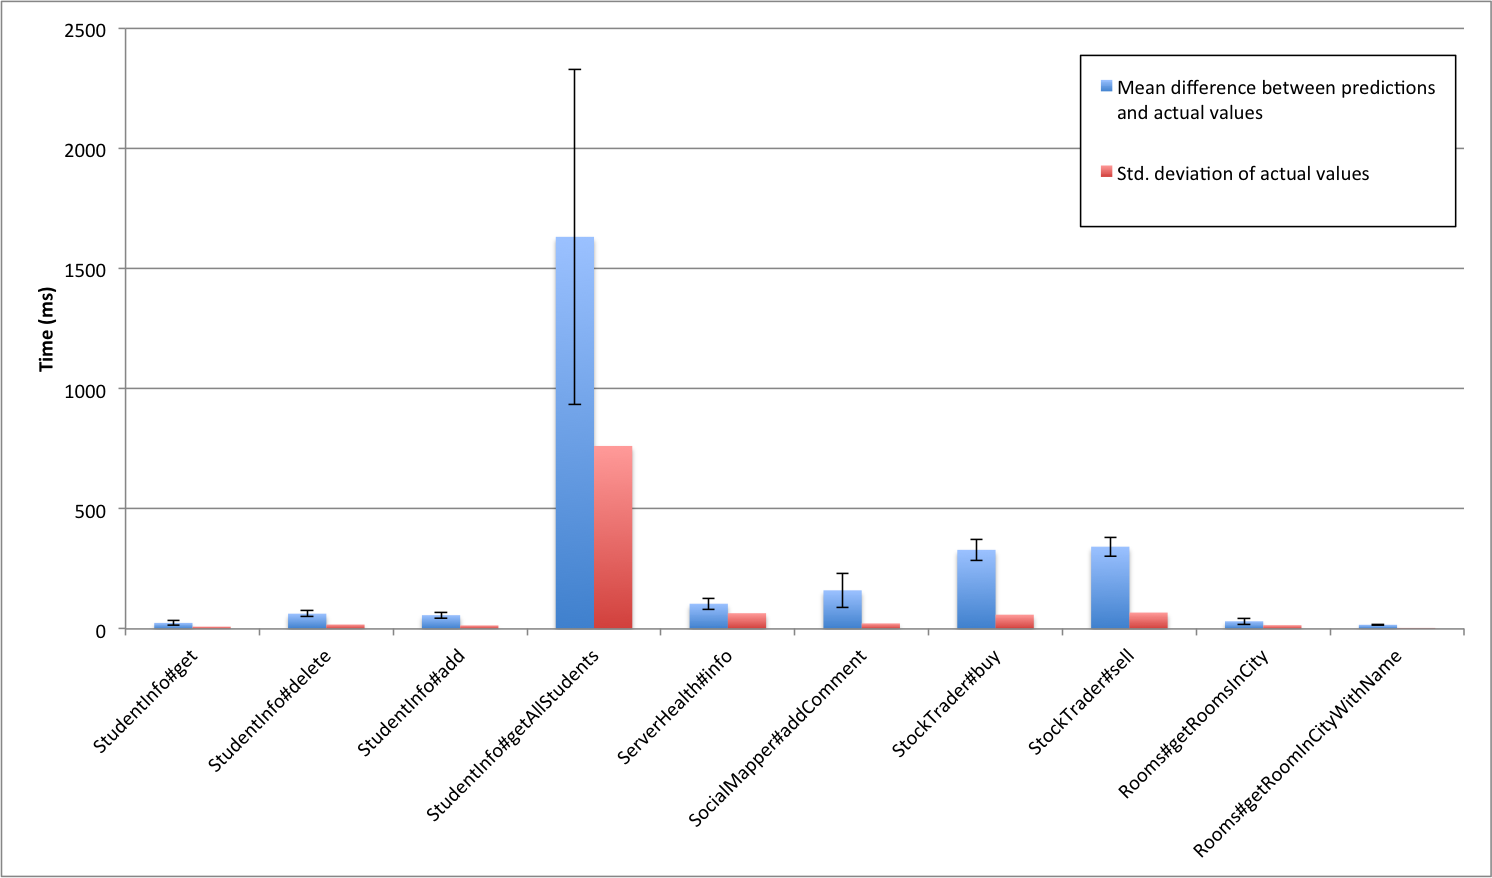
\includegraphics[scale=0.35]{gae_mean_diff}
\caption{Average difference between predictions and actual response times in Google App Engine.}
\label{fig:gae_mean_diff}
\end{figure}

Figure~\ref{fig:gae_mean_diff} depicts the average difference between predicted response times and actual response times for
our sample web APIs when running in the Google App Engine cloud. These values 
were computed considering a sequence of 1000 consecutive predictions (of 95th percentile) made by Cerebro. Within these sequences only the cases 
where the predicted value was larger than the corresponding actual value was taken into account. Based on our previous results
concerning the percentage accuracy, we know that this case occurs at least 95\% of the time.